%!TEX spellcheck=ro_RO
%!TEX root = ./main.tex
\chapter{Prezentarea aplicației}\label{ch:3implementare}
Scopul lucrării îl constituie folosirea paradigmei învățării automate supervizate, mai precis, utilizarea rețelelor neuronale convoluționale pentru clasificarea a trei stări mentale diferite, \textit{neutru, relaxat} și \textit{concentrat}. Datele aferente fiecărei stări provin de la un dispozitiv comercial, \textit{Muse 2016}, capabil de a înregistra activitatea cerebrală folosind tehnica de imagistică \textit{EEG (Electroencefalografia)}, neinvazivă. Aceste înregistrări reprezintă activitatea creierului din jurul electrozilor dispusă în timp. Deoarece dispozitivul folosit folosește o tehnică neinvazivă cu electrozi uscați datele finale ale înregistrării conțin zgomot produs de mișcările persoanei, de contracțiile mușchilor sau chiar de clipit. Din aceste motive datele trebuie prelucrate. Este de menționat faptul că nu există o anumită formulă de prelucrare pentru ca datele sa fie perfecte pentru etapa de clasificare, metodele folosite în această etapă fiind stabilite adesea empiric. După prelucrarea datelor, urmează un pas de extragere a anumitor atribute/caracteristici statistice și spectrale pe baza cărora vor fi construite imaginile alb-negru. Fiecare imagine va avea o etichetă aferentă clasei din care face parte, neutru, relaxat sau concentrat.

După etapa de prelucrare și etichetare a datelor, urmează pregătirea datelor pentru transformarea acestora sub forma unor imagini alb-negru. Această etapă include selectarea celor mai relevante 400 de atribute, dintr-un total de 414. Pentru a putea fi folosite ca și componente ale unei imagini alb-negru, este necesară normalizarea datelor în intervalul $[0,1]$, 0 reprezentând negru, 1 reprezentând alb, orice altă valoare aparținând intervalului reprezentând o nuanță de gri. Imaginile sunt împărțite apoi în diferite seturi, fiecare cu scopul său specific; setul de antrenare, setul de validare și setul de testare. Antrenarea rețelei convoluționale se realizează folosind setul de antrenare și setul de validare pentru evaluarea performanțelor pe parcursul antrenării. În final, setul de testare este folosit pentru a determina performanța rețelei pe date complet noi, rezultând metricile finale, precum acuratețea sau valoarea funcției de cost \textit{(loss)}. În cazul rețelei dezvoltate în această lucrare a fost atinsă o acuratețe de $\approx92\%$ cu valoarea funcției de loss de $\approx0.27$. 

În continuarea capitolului, etapele prezentate sumar anterior vor fi detaliate și explicate, urmând ca la finalul capitolului să fie prezentate rezultatele implementării.

\section{Etape implementare}

\subsection{Achiziție date}\label{subsec:achizitie-date}
Pentru achiziția datelor a fost folosită casca comercial valabilă Muse 2016. Interfațarea acesteia cu calculatorul a fost realizată folosind biblioteca \textit{MuseLSL} \cite{online:muselsl}, pentru limbajul de programare \textit{Python}. Această bibliotecă oferă posibilitatea conectării căștii Muse 2016, prin Bluetooth, cu calculatorul pentru transmisia de date, salvarea acestora în fișiere sau afișarea sub forma unui grafic.

Casca Muse 2016 conține cinci electrozi uscați, unul fiind folosit ca punct de referință, iar ceilalți patru pentru a înregistra semnalele EEG. Electrozii sunt poziționați în locațiile \textit{TP9, AF7, Fpz, AF8, TP10}, conform unei versiuni modificate a sistemului internațional 10-20 de poziționare al electrozilor EEG. Electrodul Fpz este folosit ca electrod de referință. În \autoref{fig:eegstandard} este prezentat aranjamentul electrozilor.

\begin{figure}[ht]
\centering
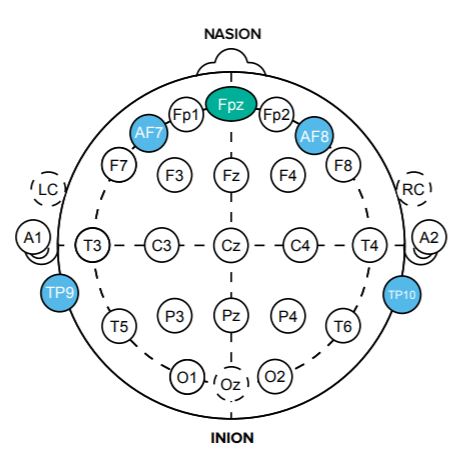
\includegraphics[width=10cm, keepaspectratio]{fig/cap3/EEGstandard.png}
\caption{Versiunea modificată a sistemului internațional 10-20 împreună cu marcajul poziției electrozilor căștii Muse \cite{online:muse-eeg}}
\label{fig:eegstandard}
\end{figure}

Pentru a diminua zgomotul înregistrat de senzori, pentru fiecare stare au fost alese activități care necesitau o mișcare minimă a persoanei examinate. Citirile datelor de la electrozii AF7 și AF8, fiind situați pe frunte, sunt distorsionate de mișcările generate de clipit. Astfel, pentru a păstra o uniformitate asupra celor trei stări, clipitul nu a fost nici încurajat nici descurajat. Chiar dacă acesta este considerat zgomot, rata de clipire este influențată de starea de concentrare a persoanei, acest lucru fiind util în final pentru algoritmul de clasificare. Totuși, persoanelor examinate le-a fost specificat să nu inchidă ochii pe durata unui test.

Pentru determinarea celor trei stări mentale, au fost stabilite trei activități, conform \cite{eeg:2018}. Pentru înregistrarea stării neutre, participanții au fost îndrumați să păstreze o poziție confortabilă a corpului și o stare mentală echilibrată, nici prea relaxată dar nici prea activă. Înregistrarea stării mentale de relaxare a presupus ca subiecții să asculte o piesă muzicală cu o tonalitate și un tempo scăzut. Acestora le-a fost indicat faptul de a se relaxa complet, atât fizic cât și psihic. Pentru determinarea stării mentale active și concentrate participanții au fost instruiți să joace o variantă a jocului „alba-neagra”, în care un obiect este ascuns sub unul din mai multe pahare, care mai apoi sunt amestecate între ele. Scopul jocului fiind de a identifica paharul care conține obiectul. Pe parcursul jocului, numărul paharelor și viteza cu care acestea se mișcă crește.

Activitățile au fost desfășurate începând cu starea neutră, urmată de starea de relaxare, iar la final starea de concentrare. Pentru fiecare activitate în parte au fost efectuate două înregistrări ale datelor EEG pe o durată de 65 de secunde. Primele 3 și ultimele 2 secunde fiind șterse ulterior, scopul acestora fiind de a crea o zonă de tranziție. Datele EEG au fost colectate de la 12 persoane, 5 de sex feminin, 7 de sex masculin. În total au fost înregistrate 26 de minute per stare, din care 24 de minute utilizabile. În \autoref{fig:muse_eeg_sample} pot fi observate semnalele provenite de la fiecare electrod în parte. Casca oferă posibilitatea de a adăuga un senzor în plus, semnalul acestuia fiind transmis prin canalul RightAUX. Semnalul provenit de la canalul în cauză a fost eliminat deoarece nu avea conectat un senzor, transmițând astfel doar zgomot.

\begin{figure}[ht]
\centering
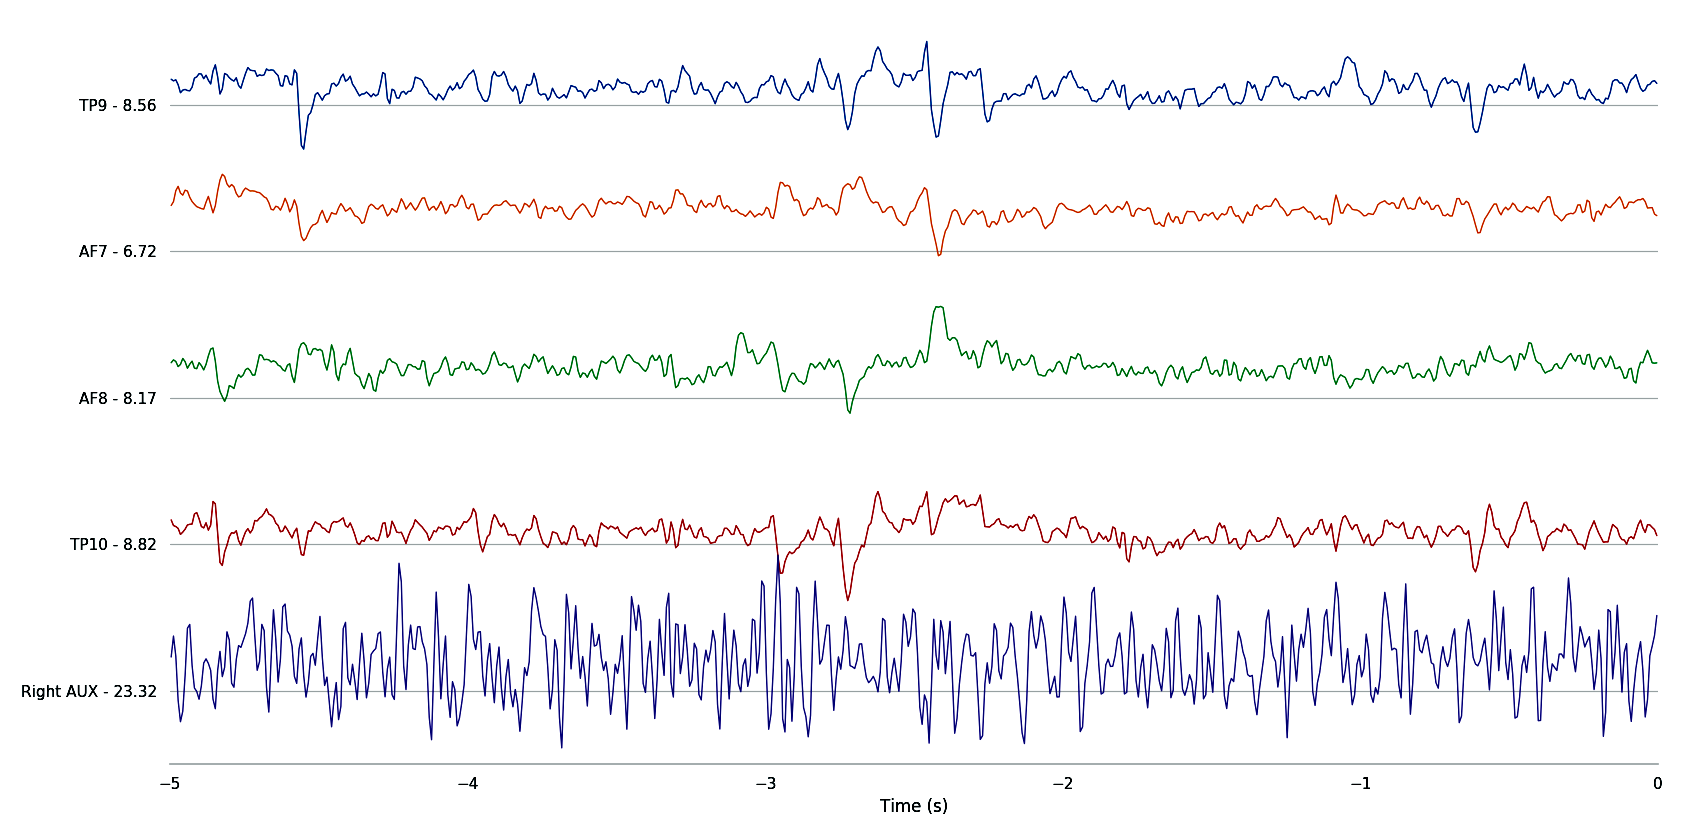
\includegraphics[width=\textwidth, keepaspectratio]{fig/cap3/museEEGplot.png}
\caption{Exemplu semnale EEG Muse 2016, extrase folosind librăria MuseLSL}
\label{fig:muse_eeg_sample}
\end{figure}

\subsection{Extragerea atributelor} 
Etapa de extragere a atributelor are rolul de a crea un set de date bazat pe semnalele EEG înregistrate, cu scopul de a fi cât mai informative pentru obiectul lucrării. Astfel, se elimină informația redundantă și nesemnificativă obiectivului, aducând avantaje precum scăderea timpului de învățăre a rețelei și o mai bună generalizare a datelor de către aceasta.

Prin set de date se înțelege o matrice de $N$ linii și $M$ coloane. Cele $M$ coloane reprezintă atributele semnalelor, 414 la număr în această lucrare, iar cele $N$ linii reprezintă valorile calculate pentru fiecare atribut în parte, 8568 în total.

În această lucrare, pe baza semnalelor EEG au fost determinate două seturi de date folosind atributele statistice ale semnalelor, respectiv atribute spectrale ale acestora. Prin atribute statistice se înțelege un set de caracteristici de natură statistică, precum media, deviația standard, varianța etc. Prin atribute spectrale se înțelege un set de caracteristici legate de spectrul semnalului EEG. Această maniera de abordare a informației conținute de semnalele EEG, precum și modul de obținere a acestor seturi de date se bazează pe cele prezentate în lucrările \cite{eeg-cnn:2020} și \cite{eeg:2018}.

Pentru calculul atributelor, semnalul a fost împărțit în „ferestre”, notate $w_i$, conținând un set de $N$ valori ale semnalului pentru durata de 1 secundă, transmise cu frecvența $256\si{\hertz}$. Ferestrele conțin o suprapunere de 0.5 secunde, astfel $w_1=[0,1]$, $w_2=[0.5,1.5]$, $w_3=[1,2]$, etc. Din fiecare fereastră rezultată au mai fost create, prin împărțirea fiecărei ferestre $w_i$, jumătăți și sferturi de fereastră. Rezultă, astfel, $w_{h1}$ și $w_{h2}$, reprezentând prima respectiv a doua jumătate a ferestrei, fiecare conținând $N/2$ valori, iar $w_{q1}$, $w_{q2}$, $w_{q3}$, $w_{q4}$ reprezentând sferturile ferestrei, fiecare conținând $N/4$ valori.

\subsubsection*{Atribute statistice}
Având aceste ferestre create, pentru fiecare fereastră $w_i$ au fost extrase atribute statistice considerând fie întreaga fereastră, fie jumătățile, fie sferturile. Astfel, pentru fiecare semnal EEG, au fost extrase următoarele atribute:
\begin{itemize}
	\item Considerând o întreagă fereastra, $w$:
	\begin{enumerate}
	\item Media valorilor ferestrei
	\begin{equation}
	\mu = \frac{1}{N}\sum_n^N x_n
	\label{eq:mean}
	\end{equation}
	unde $x$ reprezintă setul de valori dintr-o fereastră
	\item Deviația standard a valorilor
	\begin{equation}
	\sigma = \sqrt{\frac{1}{N}\sum_n^N(x_n - \mu)^2}
	\end{equation}
	\item Varianța (dispersia) valorilor
	\begin{equation}
	\sigma^2 = \frac{1}{N}\sum_n^N(x_n - \mu)^2
	\end{equation}
	\item Momentul centrat de ordin 3 (asimetria valorilor) 
	\begin{equation}
	\mu_3 = \frac{1}{N}\sum_n^N(x_n - \mu)^3
	\end{equation}
	\item Momentul centrat de ordin 4 (aplatizarea valorilor)
	\begin{equation}
	\mu_4 = \frac{1}{N}\sum_n^N(x_n - \mu)^4
	\end{equation}
	\item Covarianța perechilor de semnale EEG (TP9, AF7, AF8, TP10)
	\begin{equation}
	cov(X,Y) = \frac{1}{N}\sum_n^N(x_n - \mu_x)(y_n - \mu_y)
	\end{equation}
	unde $x$ și $y$ reprezintă setul de valori dintr-o fereastră a unui semnal EEG, iar $\mu_x$ și $\mu_y$ reprezintă media acestora calculată conform \eqref{eq:mean}
	\item Valoarea maximă și valoarea minimă a ferestrei
	\end{enumerate}
	\item Considerând jumătățile de fereastră, $w_{h1}$ și $w_{h2}$:
	\begin{enumerate}
		\item Diferența dintre media valorilor jumătăților
		\item Diferența dintre deviația standard a valorilor jumătăților
		\item Diferența dintre maximul valorilor jumătăților
		\item Diferența dintre minimul valorilor jumătăților
	\end{enumerate}
	\item Considerând sferturile de fereastră, $w_{q1}$, $w_{q2}$, $w_{q3}$, $w_{q4}$:
		\begin{enumerate}
		\item Media valorilor sferturilor de fereastră
		\item Diferența mediilor perechilor de ferestre
		\item Valoarea maximă și valoarea minimă a ferestrelor
		\item Diferența maximelor perechilor de ferestre
		\item Diferența minimelor perechilor de ferestre
	\end{enumerate}
\end{itemize}

La final, combinând atributele pentru fiecare semnal în parte, rezultă un total de 174 de atribute statistice.

\subsubsection*{Atribute spectrale}
Comparativ cu atributele statistice, generarea atributelor spectrale a fost făcută doar pe ferestre întregi, $w_i$. În cadrul extragerii atributelor spectrale a fost efectuată o prelucrare a semnalului înainte de a calcula atributele. A fost necesară o procesare inițială a acestora datorită zgomotului introdus semnalului util prin înregistrare. Inițial, a fost realizată o centrare a întregului semnalului în jurul valorii $0$, iar mai apoi a fost aplicat un filtru trece-jos de tip Chebyshev I (Fig. \ref{fig:cheb1-filt}), cu frecvența de tăiere de $50\si{\hertz}$. A fost folosit acest filtru datorită proprietăților sale de a oferi o bandă de tranziție mai îngustă dar cu introducerea unui riplu acceptabil în banda de trecere. Riplul maxim admis folosit în implementarea filtrului a fost de $0.5\%$. Prin această filtrare se păstrează doar banda de frecvență relevantă undelor cerebrale, anume $1-50\si{\hertz}$.
\begin{figure}[ht]
\centering
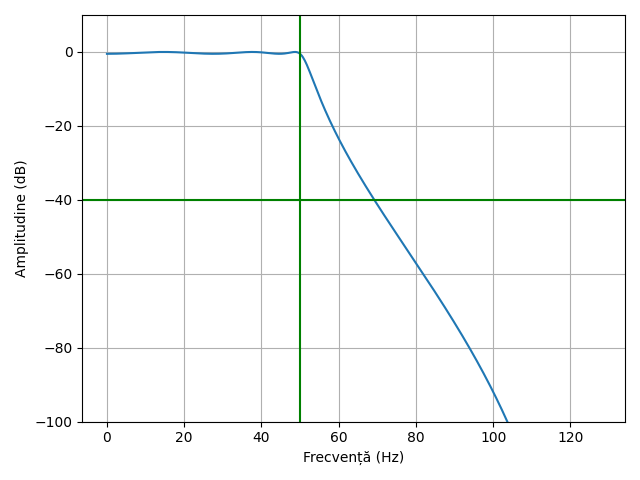
\includegraphics[width=\textwidth, keepaspectratio]{fig/cap3/cheb1-filt.png}
\caption{Răspunsul în frecvența a filtrului trece-jos de tip Chebyshev I de ordin 6}
\label{fig:cheb1-filt}
\end{figure}

După aplicarea filtrului asupra întregului semnal EEG, a fost calculată Transformata Fourier Discretă \textit{(DFT)}, folosind algoritmul \textit{Fast Fourier Transform (FFT)}. Apoi, au fost extrase amplitudinile fiecărei componente spectrale ale semnalului filtrat, rezultând 50 de atribute per semnal. Ultimele atribute extrase au fost amplitudinile celor mai puternice 10 frecvențe din componența semnalului. Acestea au fost ordonate crescător în funcție de frecvența semnalului. În total, au rezultat 240 de atribute.

Combinând cele 174 de atribute statistice cu aceste 240 de atribute spectrale, rezultă un total de 414 atribute. La setul de date format de acestea, se adaugă și o etichetă reprezentând clasa fiecărei înregistrări (0 - neutru, 1 - concentrat, 2 - relaxat). Prin procesarea celor 24 de minute pentru fiecare stare, rezultă un set de date final cuprins din 8568 de linii, reprezentând ferestrele procesate și 415 coloane reprezentând atributele și clasa fiecărei ferestre. Ultimul pas a fost de a amesteca intrările setului de date creat pentru a-l omogeniza.

\subsubsection*{Procesarea setului de date}\label{ssch:procesare-date}
După crearea setului de date, acesta trece printr-o serie de modificări înainte de a fi folosit ca și intrare pentru rețeaua convoluțională. Pentru a putea trimite datele rețelei, este necesar ca acestea să fie sub formă matriceală. Cea mai mare matrice pe care o putem forma este o matrice de dimensiunea $20\times20$, folosind doar 400 din cele 414 atribute ale acestui set de date. Această cerință impune folosirea unui algoritm pentru selecția celor mai semnificative atribute.

Selecția atributelor a fost făcută folosind \textit{testul chi-pătrat ($\chi^2$) al asocierii} \cite{online:chi-squared-pdf}, care măsoară asocierea a două variabile cu scopul de a determina o relație între acestea. Pentru comparație, a mai fost folosită metoda \textit{Informației Mutuale} \cite{online:info-mutuala}. Aceasta măsoară dependența dintre două variabile, determinând cantitatea de informație furnizată de o variabilă cu privire la alta.

Pe setul de date rezultat după aplicarea algoritmului de selecție este aplicată o scalare a fiecărei înregistrare, prin procedura de \textit{scalare min-max} care comprimă valorile în intervalul $[0,1]$. Imaginile rezultate se pot observa în \autoref{fig:img-dataset}. După aceste procesări, datele au fost transformate din dimensiunea $1\times400$ într-o matrice pătratică de dimensiunea $20\times20\times1$. Ultima dimensiune reprezentând numărul de canale al imaginii. Imaginea fiind alb-negru conține un singur canal. Ultima etapă înainte de a trimite datele rețelei este de a împărți setul de date în trei seturi distincte, pentru antrenare, validare și testare. Din totalul de date valabile, $\approx72\%$ sunt folosite ca și date de antrenare, $\approx18\%$ ca și date de validare, iar restul de $\approx10\%$ pentru testarea finală. 
\begin{figure}[ht]
\centering
\subfloat[Imagini reprezentând starea neutră]{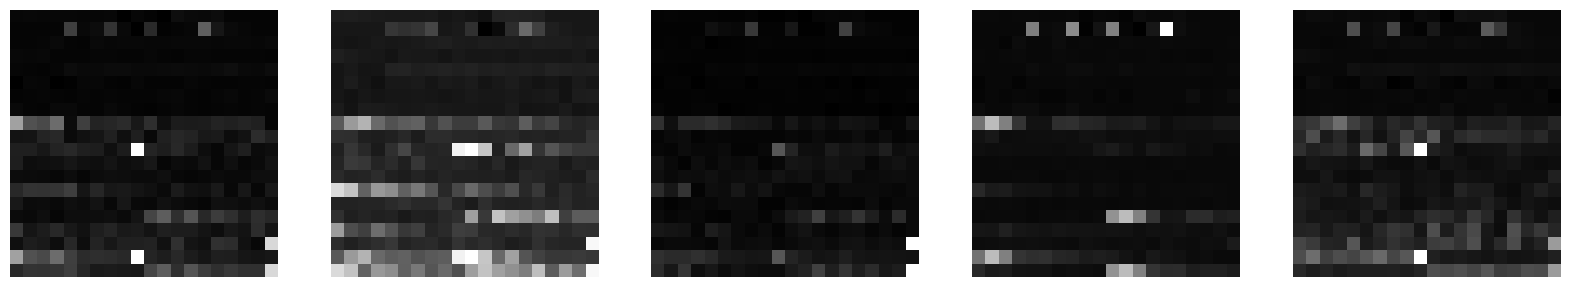
\includegraphics[width=12cm, keepaspectratio]{fig/cap3/neutral-imgs.png}\label{fig:neutral-imgs}}
\qquad
\subfloat[Imagini reprezentând starea concentrată]{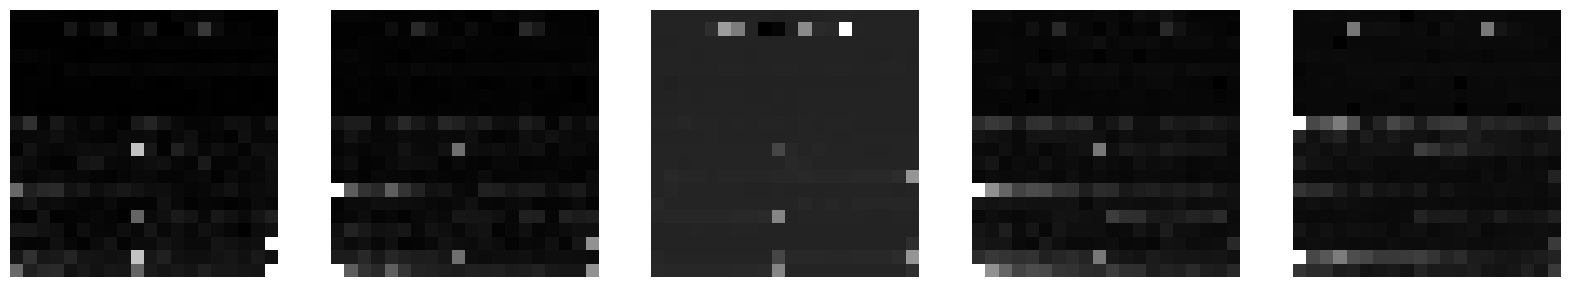
\includegraphics[width=12cm, keepaspectratio]{fig/cap3/focused-imgs.png}\label{fig:focused-imgs}}
\qquad
\subfloat[Imagini reprezentând starea relaxată]{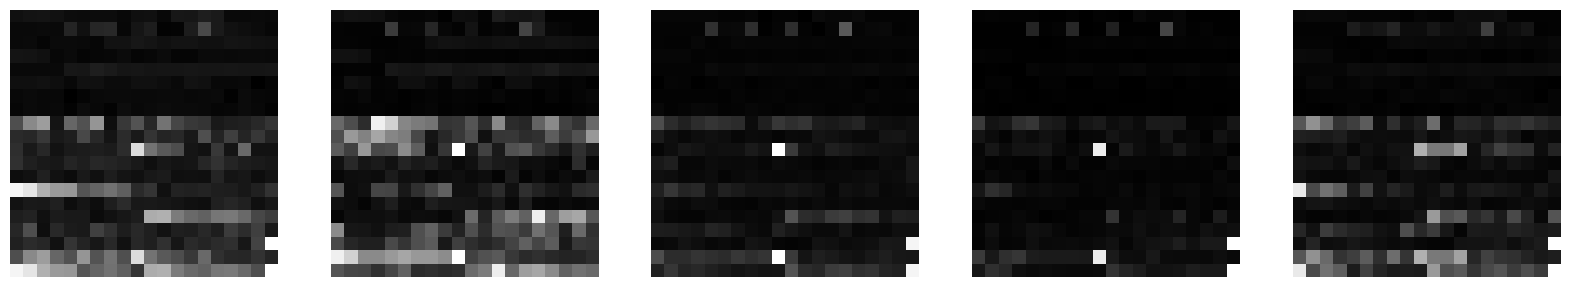
\includegraphics[width=12cm, keepaspectratio]{fig/cap3/relaxed-imgs.png}\label{fig:relaxed-imgs}}
\caption{Reprezentarea intrărilor din setul de date sub forma unor imagini alb-negru}\label{fig:img-dataset}
\end{figure}

\subsection{Arhitectura rețelei convoluționale}
Arhitectura rețelei este compusă dintr-un total de 15 straturi secvențiale, 6 straturi de convoluție, 3 straturi de normalizare, 3 straturi de \textit{dropout}, 1 strat de aplatizare și 2 straturi complet conectate, având următoarele funcții:
\begin{itemize}
\item \textbf{Conv2D:} Reprezintă stratul de convoluție, cu rolul de a învăța harta de caracteristici. Dimensiunea tuturor filtrelor folosite în această rețea este de $2\times2$. Pentru reducerea dimensionalității a fost folosit, în stratul 3 și stratul 5 de convoluție, pasului (stride) cu valoarea 2. Tuturor straturilor le-a fost aplicată funcția de activare ReLU \eqref{eq:relu}
\item \textbf{BatchNormalization \textnormal{\cite{ioffe2015batch}}:} Acest strat are rolul de a aplica o metodă de normalizare a datelor de intrare, reducând media acestora la $\approx0$, iar varianța la $\approx1$. Printre efectele acestei operații se numără accelerarea învățării rețelei neuronale și prevenirea efectului de \textit{overfitting}, care reprezintă o învățare prea bună a datelor de antrenare de către rețea, eșuând atunci când vine vorba de o clasificare a unor date noi
\item \textbf{Dropout \textnormal{\cite{hinton2012improving-dropout}}:} Stratul dropout elimină conexiunile dintre straturi, într-o anumită proporție, pentru a „forța” rețeaua de a se adapta și de a generaliza datele de intrare. Prin acest procedeu se reduce fenomenul de \textit{overfitting}
\item \textbf{Flatten:} Acest strat are rolul de a „aplatiza” matricea provenită de la ultimul strat convoluțional, transformând-o într-un vector coloană de dimensiunea $(M*N*C)\times1$, unde $M$ este numărul de linii, $N$, numărul de coloane, iar $C$ numărul de filtre
\item \textbf{Dense:} Reprezintă straturile complet conectate, specifice unei rețele neuronale, cu rolul în clasificarea datelor procesate de către partea convoluțională a rețelei. Ultimul strat conține funcția de activare \textit{softmax} (\S\ref{subsec:strat-complet-con}), specifică clasificării multi-clasă
\end{itemize}

\autoref{tabel:cnn-arch} prezintă structurat arhitectura rețelei convoluționale implementate. Este util de menționat faptul că primul element din componența dimensiunilor datelor de intrare și ieșire reprezintă dimensiunea grupului de date trimis (\textit{batch size}, explicat în \S\ref{ssch:antrenarea}). Aceasta se notează cu 0 sau \textit{None}, fiind o variabilă necunoscută în momentul implementării arhitecturii. Rețeaua convoluțională a fost implementată folosind biblioteca \textit{Keras}, conținută în framework-ul \textit{TensorFlow} \cite{online:tf-keras}.

\begin{longtable}{@{}c*4l@{}}
\renewcommand{\arraystretch}{1.2}\\
\caption{Arhitectura rețelei convoluționale implementate}\label{tabel:cnn-arch}\\
\rowcolor{gray!50}
\# & Strat & Intrare & Ieșire & Parametri \\
\endfirsthead
\rowcolor{gray!50}
\# & Strat & Intrare & Ieșire & Parametri \\
\endhead
1 & Conv2D (ReLU) & (0, 20, 20, 1) & (0, 20, 20, 32) & 160 \\
2 & Conv2D (ReLU) & (0, 20, 20, 32) & (0, 19, 19, 32) & 4128 \\
3 & BatchNormalization & (0, 19, 19, 32) & (0, 19, 19, 32) & 128 \\
4 & Dropout (0.3) & (0, 19, 19, 32) & (0, 19, 19, 32) & 0 \\
5 & Conv2D (ReLU) & (0, 19, 19, 32) & (0, 10, 10, 64) & 8256 \\
6 & Conv2D (ReLU) & (0, 10, 10, 64) & (0, 9, 9, 64) & 16448 \\
7 & BatchNormalization & (0, 9, 9, 64) & (0, 9, 9, 64) & 256 \\
8 & Dropout (0.25) & (0, 9, 9, 64) & (0, 9, 9, 64) & 0 \\
9 & Conv2D (ReLU) & (0, 9, 9, 64) & (0, 4, 4, 128) & 32896 \\
10 & Conv2D (ReLU) & (0, 4, 4, 128) & (0, 3, 3, 256) & 131328 \\
11 & BatchNormalization & (0, 3, 3, 256) & (0, 3, 3, 256) & 1024 \\ \midrule
12 & Flatten & (0, 3, 3, 256) & (0, 2304) & 0 \\
13 & Dense (ReLU) & (0, 2304) & (0, 256) & 590080 \\
14 & Dropout (0.5) & (0, 256) & (0, 256) & 0 \\
15 & Dense (softmax) & (0, 256) & (0, 3) & 771 \\ \bottomrule
\end{longtable}

\subsection{Antrenarea rețelei}\label{ssch:antrenarea}
Antrenarea rețelei a fost realizată folosind mediul online \textit{Google Colaboratory}, care pune la dispoziție atât resurse hardware cât și software specializate pentru dezvoltarea algoritmilor de învățare automată. Resursele hardware folosite pentru antrenare au fost: placa grafică NVidia Tesla K80, procesorul Intel Xeon @ 2.00 GHz și 13GB RAM. Folosind aceste resurse, timpul total de antrenare al rețelei a fost de aproximativ 3 secunde per epocă.

Antrenarea a fost realizată folosind:
\begin{itemize}
\item Funcția de cost: \textit{Categorical Cross-Entropy}, folosită în problemele de clasificare multi-clasă, se folosește în conjuncție cu funcția de activare \textit{softmax} de la ieșirea rețelei pentru a calcula un vector de probabilități de dimensiunea numărului de clase \cite{online:CCE-loss}. Clasa fiecărei înregistrări este codată folosind tehnica \textit{one-hot encode} care presupune scrierea clasei sub forma unui vector care conține valoarea 1 la poziția specificată de clasa reprezentată, restul fiind 0, de exemplu $[0,1,0]$ pentru clasa 1. Astfel, doar scorul obținut pentru clasa respectivă va fi folosit în calcului valorii de \textit{loss/cost}
\item Funcția de optimizare: Pentru optimizarea funcției de cost a fost folosită funcția \textit{Adam} \cite{kingma2014adam}, folosind o rată de învățare inițială $\eta=7*10^{-4}$ și reducerea acesteia cu factorul $7*10^{-2}$ dacă valoarea funcției de cost nu se îmbunatățește pentru o perioadă de 5 epoci, până la valoarea minimă $10^{-5}$
\end{itemize}

Modelul realizat a fost antrenat pentru o perioadă de 100 de epoci, folosind un \textit{grup (batch size)} de 32 de imagini. Epoca este perioada de timp în care toate înregistrările conținute în setul de antrenare sunt trecute prin rețea. \textit{Batch size} reprezintă o serie/grup de înregistrări pe care rețeaua le ia în considerare înainte de a-și modifica parametrii. Prin folosirea unor serii în detrimentul unei singure înregistrări, capacitatea de generalizare a informației de către rețeaua antrenată crește, rezultând o mai bună adaptare către noi date. Acest procedeu permite folosirea calculului paralel, prin distribuirea înregistrărilor pe mai multe fire de execuție rezultând un timp de antrenare al rețelei mai scăzut. 

\section{Rezultate}
În această secțiune sunt prezentate rezultatele obținute de modelul rețelei convoluționale implementate. În \autoref{tabel:acc+loss+comparison} sunt prezentate comparativ rezultatele obținute în urma antrenării modelului rețelei convoluționale implementate pe setul de date creat, folosind ca algoritm de selecție al atributelor pe rând două metode: metoda de testare \textit{chi-pătrat}, iar mai apoi metoda \textit{informației mutuale}. Testele comparative au fost realizate de 3 ori pentru fiecare metodă, folosind setul de test.

\begin{table}[h]
\centering
\caption{Prezentarea performanțelor modelului folosind metodele \textit{chi-pătrat} și \textit{informație mutuală} (\S\ref{ssch:procesare-date}) pentru selecția atributelor}
\label{tabel:acc+loss+comparison}
\renewcommand{\arraystretch}{1.2}
\begin{tabular}{@{}llcc@{}}
\rowcolor{gray!50} Metodă & \# & Valoare loss & Valoare acuratețe \\ 
& 1 & 0.268 & 0.931 \\
Chi pătrat & 2 & 0.278 & 0.919 \\
& 3 & 0.269 & 0.924 \\
\rowcolor{gray!15} Media & & 0.272 & 0.925 \\
& 1 & 0.283 & 0.928 \\{}
Informație & 2 & 0.282 & 0.920 \\
mutuală & 3 & 0.282 & 0.927 \\
\rowcolor{gray!15} Media & & 0.282 & 0.925 \\
\end{tabular}
\end{table}

Rezultatele inițiale obținute fiind foarte asemanatoare, am decis folosirea metodei chi-pătrat pentru selecția atributelor. Toate rezultatele prezentate în continuare reies din setul de date format prin această metodă.

Evoluția pe perioada antrenării a acurateței și a valorii funcției de cost poate fi observată în \autoref{fig:acc+loss+graph}. Colorat cu albastru este reprezentată acuratețea/valoarea funcție de cost a modelului provenite din analizarea performanțelor acestuia pe setul de antrenare. Cu portocaliu este reprezentată performanța acestuia în clasificarea datelor din setul de validare. Deoarece modelul își ajustează parametrii, în cea mai mare măsură, în funcție de setul de antrenare, metricile rezultate pentru acest set vor fi întotdeauna mai bune decât metricile calculate pe restul seturilor de date. Pe parcursul antrenării, la finalul fiecărei epoci, setul de validare este folosit pentru evaluarea modelului și ajustarea parametrilor acestuia. 

Urmărind cele două grafice putem observa faptul că evoluția metricilor modelului calculate pe setul de validare este foarte apropiată de cele calculate pe setul de antrenare. Acest lucru sugerează o performanța bună a clasificatorului, acesta fiind capabil să generalizeze datele primite la învățare și să aplice aceste „cunoștiințe” pentru a clasifica cât mai corect posibil date pentru care nu este antrenat în mod direct. Din aceste grafice mai poate fi observată utilitatea modificării ratei de învățare. La epoca 36, rata de învățare se diminuează cu $0.07$ ajungând de la $7*10^{-4}$ la valoarea $4.9*10^{-5}$, crescând acuratețea modelului și diminuând valoarea funcției de cost. Este posibil ca acest lucru să se fi întâmplat și fară a face această operațiune, însă pe o perioadă de timp mult mai lungă, crescând timpul total de învățare.

După finalizarea antrenării modelului, capacitățile acestuia au fost testate asupra setului de date de test, date pe care acesta nu le „văzuse” niciodată. Evaluarea a fost efectuată de trei ori, rezultând o acuratețe medie de $\approx92\%$ și o valoarea medie a funcție de cost de $\approx0.2$.
\begin{figure}[H]
\centering
\subfloat[]{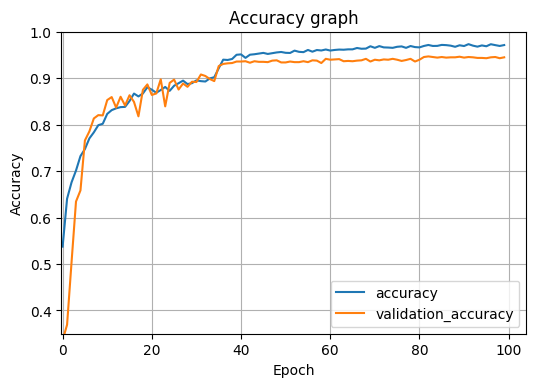
\includegraphics[width=6.9cm, keepaspectratio]{fig/cap3/acc_graph.png}\label{fig:acc_graph}}
\qquad
\subfloat[]{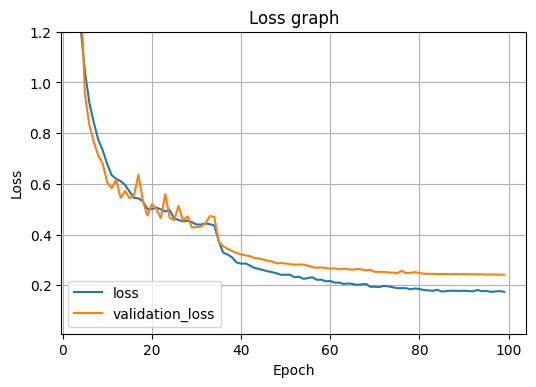
\includegraphics[width=6.9cm, keepaspectratio]{fig/cap3/loss_graph.png}\label{fig:loss_graph}}
\caption{Reprezentările grafice ale evoluției acurateței modelului \protect\subref{fig:acc_graph} și evoluției valoarii funcției de cost \protect\subref{fig:loss_graph}}\label{fig:acc+loss+graph}
\end{figure}

Pentru determinarea performanțelor, pe lângă acuratețea modelului și valoarea funcției de cost, au mai fost calculate următoarele metrici, valorile rezultate sunt prezentate în \autoref{tabel:classification-report}:
\begin{itemize}
\item Precision: reprezintă precizia clasificatorului, fiind determinată de proporția cazurilor \textit{true positive} din totalitatea prezicerilor clasificate ca aparținând de clasa adevărată (suma clasificărilor \textit{true positive} și \textit{false positive})
\item Recall: reprezintă „rata de regăsire„ a clasificatorului, fiind determinată de proporția cazurilor \textit{true positive} din totalitatea prezicerilor care aparțin cu adevărat de clasa respectivă (suma clasificărilor \textit{true positive} și \textit{false negative})
\item $F_\beta$ Score: reprezintă o media armonică ponderată între precision și recall. Dacă ponderea $\beta$ are valoarea 1, cele două metrice sunt luate în considerare în aceeași proporție, fiind considerate la fel de importante
\end{itemize}

\begin{table}[ht]
\centering
\caption{Reprezentarea valorilor metricilor \textit{precision, recall} și \textit{$F_1$ score} pentru fiecare clasă}
\label{tabel:classification-report}
\renewcommand{\arraystretch}{1.2}
\begin{tabular}{@{}lcccc@{}}
%\cmidrule[\heavyrulewidth]{2-4}
\rowcolor{gray!50}\cellcolor{white} & Precision & Recall & $F_1$ Score \\ %\cmidrule{2-4}
neutru & 0.91 & 0.95 & 0.93 \\
concentrat & 0.97 & 0.94 & 0.93 \\
relaxat & 0.92 & 0.90 & 0.91 \\ \bottomrule
\end{tabular}
\end{table}

\autoref{fig:conf_matrix} afișează performanțele clasificatorului prin așezarea prezicerilor acesteia într-o matrice denumită Matricea Confuziilor \textit{(Confusion Matrix)}. Matricea conține pe diagonala principală toate clasificările corecte.

\begin{figure}[H]
\centering
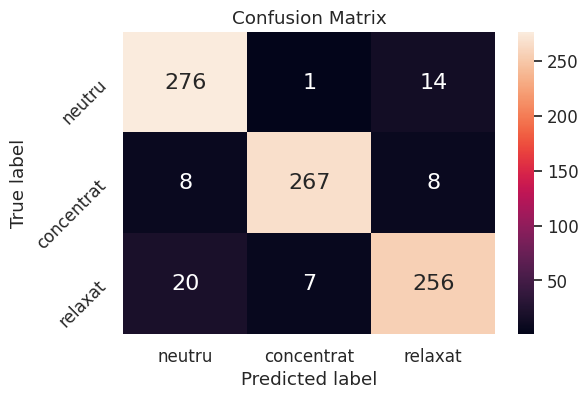
\includegraphics[width=9cm, keepaspectratio]{fig/cap3/conf_matrix.png}
\caption{Reprezentarea performanței rețelei prin matricea confuziilor}\label{fig:conf_matrix}
\end{figure}

Din datele afișate atât în \autoref{tabel:classification-report}, cât și în \autoref{fig:conf_matrix}, unde este reprezentată matricea confuziilor, poate fi observată dificultatea clasificatorului de a distinge clasele \textit{neutru} și \textit{relaxat}. Această dificultate în distingere apare datorită metodelor asemănatoare de culegere a datelor EEG pentru ambele clase, descrise în \S\ref{subsec:achizitie-date}. 
